\chapter{组合数学}
\intro{组合数学研究离散对象的计数、排列、组合与存在性问题，是离散数学的核心分支之一。}

\section{计数基本原理}

\subsection{加法原理}

\begin{mydefinition}{}
设 $A_1, A_2, \dots, A_k$ 是两两不交的有限集，则
\[
\left|\bigcup_{i=1}^{k} A_i\right| = \sum_{i=1}^{k} |A_i|
\]
\end{mydefinition}

通俗地说：若有 $k$ 项互斥的任务，第 $i$ 项有 $n_i$ 种完成方式，则从中任选一项完成共有 $n_1 + n_2 + \dots + n_k$ 种方式。

\begin{example}
某班有男生 20 人、女生 18 人，选 1 名代表，共有 $20 + 18 = 38$ 种选法。
\end{example}

\subsection{乘法原理}

\begin{mydefinition}{}
若 $A_1, A_2, \dots, A_k$ 是有限集，则
\[
|A_1 \times A_2 \times \dots \times A_k| = \prod_{i=1}^{k} |A_i|
\]
\end{mydefinition}

通俗地说：若一项任务可分解为 $k$ 个独立步骤，第 $i$ 步有 $n_i$ 种选择，则完成该任务共有 $n_1 \times n_2 \times \dots \times n_k$ 种方式。

\begin{example}
车牌号格式为"字母-字母-数字-数字"，字母用 26 个大写字母，数字用 $0$--$9$，共有 $26 \times 26 \times 10 \times 10 = 67600$ 种不同车牌。
\end{example}

\begin{example}
从 $A$ 到 $B$ 有 3 条路，从 $B$ 到 $C$ 有 4 条路，则从 $A$ 经 $B$ 到 $C$ 有 $3 \times 4 = 12$ 种走法。
\end{example}

\subsection{减法原理}

在全集 $U$ 中求满足某性质的元素个数，可以先求不具有该性质的元素个数，然后从总数中减去：
\[
|A| = |U| - |\overline{A}|
\]
这本质上是容斥原理的最简形式。

\begin{example}
从 1 到 100 中，有多少个数既不含因子 2 也不含因子 3？含因子 2 的有 $\lfloor 100/2 \rfloor = 50$ 个，含因子 3 的有 $\lfloor 100/3 \rfloor = 33$ 个，同时含因子 2 和 3（即含因子 6）的有 $\lfloor 100/6 \rfloor = 16$ 个。所以不含 2 也不含 3 的有 $100 - 50 - 33 + 16 = 33$ 个。
\end{example}

\section{排列}

\subsection{线排列（不重复排列）}

\begin{mydefinition}{}
从 $n$ 个不同元素中取出 $r$ 个（$0 \leq r \leq n$）按顺序排成一列，称为一个 \heiti{$r$-排列}，其总数记为 $P(n, r)$ 或 $P_n^r$：
\[
P(n, r) = n \cdot (n-1) \cdot (n-2) \cdots (n-r+1) = \frac{n!}{(n-r)!}
\]
\end{mydefinition}

\textbf{推导}：第一位有 $n$ 种选择，第二位有 $n-1$ 种（不能重复），……，第 $r$ 位有 $n-r+1$ 种。由乘法原理即得。

\textbf{特例}：$r = n$ 时，$P(n, n) = n!$（全排列）。约定 $0! = 1$，$P(n, 0) = 1$。

\begin{example}
5 个人排队，前 3 人领奖的安排方式有 $P(5, 3) = 5 \times 4 \times 3 = 60$ 种。
\end{example}

\subsection{可重复排列}

\begin{myTheorem}{可重复排列}
从 $n$ 个不同元素中取出 $r$ 个排成一列，允许重复选取，则排列总数为
\[
n^r
\]
\end{myTheorem}

\begin{example}
3 位数密码（每位 0--9）共有 $10^3 = 1000$ 种组合。
\end{example}

\begin{example}
$n$ 个元素的集合 $A$ 到 $m$ 个元素的集合 $B$ 的函数总数为 $m^n$（每个 $a \in A$ 有 $m$ 种映射选择）。
\end{example}

\subsection{圆排列}

\begin{myTheorem}{圆排列公式}
$n$ 个不同元素的圆排列（环形排列）数为
\[
(n-1)!
\]
\end{myTheorem}

\textbf{推导}：将 $n$ 个元素排在一个圆圈上，旋转后重合视为同一排列。首先选定一个元素固定在某位置（打破旋转对称性），剩下 $n-1$ 个元素全排列，得 $(n-1)!$。

\begin{remark}
若圆排列可以翻转（即翻转后重合视为同一），则数量为 $\frac{(n-1)!}{2}$（当 $n \geq 3$）。
\end{remark}

\begin{example}
6 个人围桌而坐，有 $(6-1)! = 120$ 种坐法。
\end{example}

\subsection{多重集的排列}

\begin{mydefinition}{}
多重集有 $k$ 种不同类型的元素，第 $i$ 种有 $n_i$ 个相同元素，总元素数 $n = n_1 + n_2 + \dots + n_k$。则多重集的排列数为
\[
\frac{n!}{n_1!\, n_2!\, \dots\, n_k!}
\]
\end{mydefinition}

\begin{example}
"MISSISSIPPI" 的字母排列数：M=1, I=4, S=4, P=2，共 11 个字母。
\[
\frac{11!}{1! \times 4! \times 4! \times 2!} = 34650
\]
\end{example}

\section{组合}

\subsection{组合数（不重复组合）}

\begin{mydefinition}{}
从 $n$ 个不同元素中取出 $r$ 个（$0 \leq r \leq n$）不计顺序组成一组，称为一个 \heiti{$r$-组合}，其总数记为 $C(n, r)$、$\binom{n}{r}$ 或 $C_n^r$：
\[
C(n, r) = \binom{n}{r} = \frac{P(n, r)}{r!} = \frac{n!}{r!\,(n-r)!}
\]
\end{mydefinition}

\textbf{推导}：每个 $r$-组合对应 $r!$ 个不同的 $r$-排列，故 $P(n, r) = r! \cdot C(n, r)$。

\begin{example}
从 10 人中选 3 人组成委员会，共有 $\binom{10}{3} = 120$ 种选法。
\end{example}

\subsection{可重复组合（隔板法）}

\begin{myTheorem}{可重复组合公式}
$n$ 种元素中选出 $r$ 个的可重复组合数为
\[
\binom{n + r - 1}{r} = \binom{n + r - 1}{n - 1}
\]
\end{myTheorem}

\textbf{隔板法证明}：将 $r$ 个相同球放入 $n$ 个不同的盒子（允许空盒）。用 $r$ 个星 $\star$ 和 $(n-1)$ 条竖线 $|$ 排列表示分配方案。总共有 $r + n - 1$ 个位置，选其中 $n-1$ 个放竖线，故有 $\binom{r+n-1}{n-1}$ 种方案。

\begin{example}
方程 $x_1 + x_2 + x_3 = 10$ 的非负整数解个数为
\[
\binom{10 + 3 - 1}{3 - 1} = \binom{12}{2} = 66
\]
\end{example}

\section{二项式定理与组合恒等式}

\subsection{二项式定理}

\begin{myTheorem}{二项式定理}
对任意实数 $x, y$ 和正整数 $n$，
\[
(x + y)^n = \sum_{k=0}^{n} \binom{n}{k} x^{n-k} y^k = \sum_{k=0}^{n} \binom{n}{k} x^k y^{n-k}
\]
\end{myTheorem}

\textbf{证明（组合意义）}：$(x+y)^n = \underbrace{(x+y)(x+y)\cdots(x+y)}_{n\text{ 个}}$，展开后每项形如 $x^{n-k}y^k$，系数等于从 $n$ 个因子中选 $k$ 个取 $y$ 的方案数 $\binom{n}{k}$。

\textbf{常用推论}（取特殊值）：
\begin{align*}
x=1, y=1 &\;\Rightarrow\; \sum_{k=0}^{n} \binom{n}{k} = 2^n \\
x=1, y=-1 &\;\Rightarrow\; \sum_{k=0}^{n} (-1)^k \binom{n}{k} = 0
\end{align*}

\subsection{杨辉三角（Pascal 三角）}

\begin{mydefinition}{Pascal 恒等式}
\[
\binom{n}{r} = \binom{n-1}{r} + \binom{n-1}{r-1} \quad (0 < r < n)
\]
\end{mydefinition}

\textbf{证明（组合意义）}：从 $n$ 个中选 $r$ 个，考虑是否包含某个固定元素：
\begin{itemize}
    \item 不包含：从其余 $n-1$ 个中选 $r$ 个，共 $\binom{n-1}{r}$ 种
    \item 包含：从其余 $n-1$ 个中选 $r-1$ 个，共 $\binom{n-1}{r-1}$ 种
\end{itemize}

下面用 TikZ 绘制杨辉三角，直观展示 Pascal 恒等式的递推结构：

\begin{center}
\begin{tikzpicture}[
    dmPascal/.style={circle, draw=blue!60, fill=blue!10, minimum size=10mm, inner sep=0pt},
    dmPascalEdge/.style={-{Stealth}, thick, gray!60}
]
\foreach \n in {0,...,6} {
    \foreach \k in {0,...,\n} {
        \pgfmathtruncatemacro{\x}{2*\k - \n}
        \pgfmathtruncatemacro{\y}{-\n}
        \node[dmPascal] at (\x*0.9, \y*1.2) {\small$\binom{\n}{\k}$};
    }
}
\foreach \n in {0,...,5} {
    \foreach \k in {0,...,\n} {
        \pgfmathtruncatemacro{\nxt}{\n+1}
        \pgfmathtruncatemacro{\xa}{2*\k - \n}
        \pgfmathtruncatemacro{\ya}{-\n}
        \pgfmathtruncatemacro{\xb}{2*\k - \nxt}
        \pgfmathtruncatemacro{\yb}{-\n-1}
        \pgfmathtruncatemacro{\xc}{2*(\k+1) - \nxt}
        \draw[dmPascalEdge] ({\xa*0.9}, {\ya*1.2+0.25}) -- ({\xb*0.9}, {\yb*1.2-0.25});
        \draw[dmPascalEdge] ({\xa*0.9}, {\ya*1.2+0.25}) -- ({\xc*0.9}, {\yb*1.2-0.25});
    }
}
\node at (0, -8.5) {\fangsong 杨辉三角：每个数是上方两数之和（Pascal 恒等式）};
\end{tikzpicture}
\end{center}

\subsection{组合恒等式}

除 Pascal 恒等式外，还有以下重要恒等式：

\textbf{对称性}：$\displaystyle \binom{n}{r} = \binom{n}{n-r}$

\textbf{朱世杰恒等式（Vandermonde 卷积）}：
\[
\sum_{k=0}^{r} \binom{m}{k} \binom{n}{r-k} = \binom{m+n}{r}
\]

\textbf{证明（组合意义）}：从 $m$ 男 $n$ 女共 $m+n$ 人中选 $r$ 人，按选出的男生数 $k$ 分类，第 $k$ 类有 $\binom{m}{k} \times \binom{n}{r-k}$ 种选法，求和即得。

其他常用恒等式：
\begin{align}
\sum_{k=0}^{n} \binom{n}{k} &= 2^n \label{eq:sum-comb} \\
\sum_{k=0}^{n} (-1)^k \binom{n}{k} &= 0 \quad (n \geq 1) \label{eq:sum-comb-alt} \\
\sum_{k=0}^{n} k \binom{n}{k} &= n \cdot 2^{n-1} \label{eq:sum-k-comb}
\end{align}

\section{鸽巢原理}

\subsection{基本形式}

\begin{myTheorem}{鸽巢原理}
若把 $n+1$ 个物体放入 $n$ 个盒子中，则至少有一个盒子包含至少 2 个物体。
\end{myTheorem}

\begin{proof}
反证法。设每个盒子至多放 1 个，则 $n$ 个盒子至多容纳 $n$ 个物体，矛盾。
\end{proof}

\begin{example}
任意 13 个人中，至少有 2 人在同一个月出生。
\end{example}

\begin{example}
从 1 到 $2n$ 中任取 $n+1$ 个数，必有两数互质（取相邻两数）。
\end{example}

\subsection{加强形式}

\begin{myTheorem}{鸽巢原理（加强形式）}
设 $q_1, q_2, \dots, q_n$ 都是正整数，若将 $q_1 + q_2 + \dots + q_n - n + 1$ 个物体放入 $n$ 个盒子，则第 1 个盒子至少有 $q_1$ 个，\textbf{或}第 2 个盒子至少有 $q_2$ 个，……，\textbf{或}第 $n$ 个盒子至少有 $q_n$ 个。
\end{myTheorem}

\textbf{推论（平均形式）}：$m$ 个物体放入 $n$ 个盒子，则至少有一个盒子包含至少 $\lceil m/n \rceil$ 个物体。

\begin{center}
\begin{tikzpicture}[
    dmBox/.style={rectangle, draw=blue!70, rounded corners, minimum width=2cm, minimum height=1.2cm, fill=blue!5},
    dmSmallBox/.style={rectangle, draw=orange!70, rounded corners, minimum width=1.5cm, minimum height=0.9cm, fill=orange!5},
    dmPigeon/.style={circle, draw=red!60, fill=red!20, minimum size=6mm, inner sep=0pt}
]
\node[dmBox, label=above:{\heiti 盒子 1}] (b1) at (0,0) {};
\node[dmBox, label=above:{\heiti 盒子 2}] (b2) at (3,0) {};
\node[dmBox, label=above:{\heiti 盒子 3}] (b3) at (6,0) {};

\foreach \i in {-0.5,-0.2,0.1,0.4} {
    \node[dmPigeon] at (\i, -0.3) {};
}
\foreach \i in {2.5,2.8,3.1} {
    \node[dmPigeon] at (\i, -0.3) {};
}
\foreach \i in {5.7,6.0,6.3} {
    \node[dmPigeon] at (\i, -0.3) {};
}

\node at (3, -1.8) {10 个鸽子放入 3 个盒子，由鸽巢原理，至少有一个盒子包含 $\lceil 10/3 \rceil = 4$ 个鸽子};
\end{tikzpicture}
\end{center}

\subsection{Ramsey 理论入门}

\begin{mydefinition}{Ramsey 数}
对任意正整数 $k, l$，存在最小的正整数 $R(k, l)$，使得任何 $R(k, l)$ 个人的群体中，要么有 $k$ 个人彼此认识，要么有 $l$ 个人彼此不认识。
\end{mydefinition}

已知结果：$R(3, 3) = 6$，$R(4, 4) = 18$，而 $R(5, 5)$ 至今未知（已知在 43 到 48 之间）。

\begin{example}
$R(3,3)=6$ 的证明：6 人中必存在 3 人彼此都认识或彼此都不认识。任取一人 $A$，其余 5 人中由鸽巢原理，至少有 3 人与 $A$ 认识或至少有 3 人与 $A$ 不认识。若 3 人与 $A$ 认识，这 3 人中若有 2 人认识，则加上 $A$ 构成 3 人彼此认识；若 3 人彼此不认识，则构成 3 人彼此不认识。
\end{example}

\section{容斥原理}

\subsection{基本形式}

两集合容斥：
\[
|A \cup B| = |A| + |B| - |A \cap B|
\]

三集合容斥：
\[
|A \cup B \cup C| = |A| + |B| + |C| - |A \cap B| - |B \cap C| - |C \cap A| + |A \cap B \cap C|
\]

\begin{center}
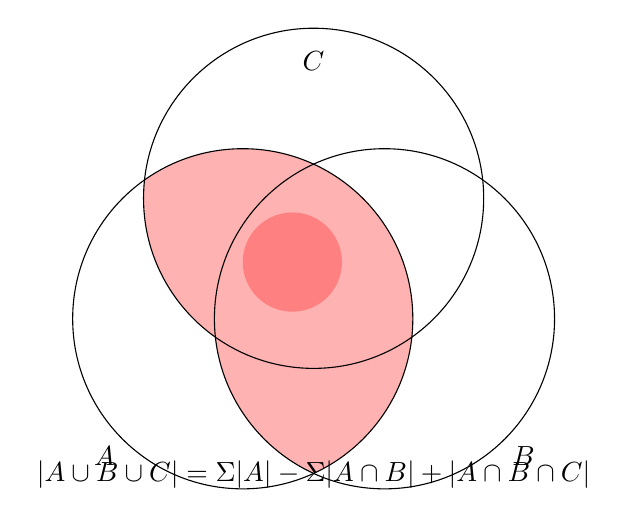
\begin{tikzpicture}[scale=1.8]
\def\circleA{(0,0) circle (1.2cm)}
\def\circleB{(1.0,0) circle (1.2cm)}
\def\circleC{(0.5,0.85) circle (1.2cm)}

\begin{scope}
    \clip \circleA;
    \fill[red!30] \circleB;
    \fill[red!30] \circleC;
    \clip \circleB;
    \fill[red!30] \circleC;
\end{scope}
\begin{scope}
    \fill[red!50] (0.35,0.4) circle (0.35cm);
\end{scope}

\draw \circleA node[below left=1.5cm] {$A$};
\draw \circleB node[below right=1.5cm] {$B$};
\draw \circleC node[above=1.5cm] {$C$};

\node at (0.5, -1.1) {$|A\cup B\cup C| = \Sigma|A| - \Sigma|A\cap B| + |A\cap B\cap C|$};
\end{tikzpicture}
\end{center}

\subsection{一般形式}

\begin{myTheorem}{容斥原理}
设 $A_1, A_2, \dots, A_n$ 是有限集 $U$ 的子集，则
\begin{align*}
\bigg|\bigcup_{i=1}^{n} A_i\bigg| = \sum_{i=1}^{n} |A_i| &- \sum_{1 \leq i < j \leq n} |A_i \cap A_j| \\
&+ \sum_{1 \leq i < j < k \leq n} |A_i \cap A_j \cap A_k| - \cdots + (-1)^{n-1} |A_1 \cap \dots \cap A_n|
\end{align*}
\end{myTheorem}

等价的补集形式（求不在任何 $A_i$ 中的元素数）更常用：
\[
\bigg|\overline{A_1} \cap \overline{A_2} \cap \dots \cap \overline{A_n}\bigg| = |U| - \sum |A_i| + \sum |A_i \cap A_j| - \cdots + (-1)^n |A_1 \cap \dots \cap A_n|
\]

\subsection{错位排列}

\begin{mydefinition}{}
$n$ 个元素的排列中，若每个元素都不在其原始位置（$a_i \neq i$），则称为一个 \heiti{错位排列}。错位排列数记为 $D_n$ 或 $!n$。
\end{mydefinition}

\begin{myTheorem}{错位排列公式}
\[
D_n = n! \sum_{i=0}^{n} \frac{(-1)^i}{i!} = n! \left(1 - \frac{1}{1!} + \frac{1}{2!} - \frac{1}{3!} + \dots + \frac{(-1)^n}{n!}\right)
\]
\end{myTheorem}

\textbf{容斥原理推导}：设 $A_i$ 为第 $i$ 个元素在正确位置的排列集合。$|A_i| = (n-1)!$，$|A_i \cap A_j| = (n-2)!$，一般地 $|A_{i_1} \cap \dots \cap A_{i_k}| = (n-k)!$。由容斥原理：
\[
D_n = n! - \sum_{k=1}^{n} (-1)^{k-1}\binom{n}{k} (n-k)! = n! \sum_{k=0}^{n} \frac{(-1)^k}{k!}
\]

\textbf{递推关系}：$D_n = (n-1)(D_{n-1} + D_{n-2})$，$D_1 = 0, D_2 = 1$。

\textbf{渐近公式}：$D_n \approx \frac{n!}{e}$（当 $n$ 较大时，约 36.79\% 的排列是错位排列）。

\begin{center}
\begin{tikzpicture}[
    dmNodeDer/.style={circle, draw=red!60, fill=red!10, minimum size=12mm, inner sep=0pt},
    level distance=2cm,
    sibling distance=2.5cm,
    edge from parent/.style={draw, -{Stealth}, thick}
]
\node[dmNodeDer] {$D_n$}
    child { node[dmNodeDer, fill=orange!10] {$D_{n-1}$}
        child { node[dmNodeDer, fill=yellow!10] {$D_{n-2}$} }
        child { node[dmNodeDer, fill=yellow!10] {$\cdots$} }
    }
    child { node[dmNodeDer, fill=orange!10] {$D_{n-2}$}
        child { node[dmNodeDer, fill=yellow!10] {$D_{n-3}$} }
        child { node[dmNodeDer, fill=yellow!10] {$\cdots$} }
    };
\node at (0, -7) [text width=10cm, align=center] {%
    \fangsong 错位排列递推结构：$D_n = (n-1)(D_{n-1} + D_{n-2})$\quad
    前几项：$D_1=0,\;D_2=1,\;D_3=2,\;D_4=9,\;D_5=44$};
\end{tikzpicture}
\end{center}

\section{递推关系入门}

\subsection{递推关系的基本概念}

\begin{mydefinition}{}
一个序列 $\{a_n\}$ 的递推关系将 $a_n$ 表示为该序列中前若干项的函数。给定初始条件，即可唯一确定整个序列。
\end{mydefinition}

\begin{example}
斐波那契数列：$F_n = F_{n-1} + F_{n-2}$，$F_0 = 0, F_1 = 1$。序列：$0, 1, 1, 2, 3, 5, 8, 13, 21, \dots$
\end{example}

\subsection{一阶线性递推}

\textbf{形式}：$a_n = c \cdot a_{n-1} + g(n)$，其中 $c$ 为常数。

\textbf{齐次情形}（$g(n) = 0$）：$a_n = c \cdot a_{n-1}$，通解为 $a_n = a_0 \cdot c^n$。

\begin{example}
汉诺塔问题：$T_n = 2T_{n-1} + 1$，$T_1 = 1$。通解：$T_n = 2^n - 1$。
\end{example}

\begin{example}
求 $n$ 位二进制串中没有连续两个 0 的个数。设 $a_n$ 为满足条件的 $n$ 位串数。递推：$a_n = a_{n-1} + a_{n-2}$（最后一位为 1 则前 $n-1$ 位任意；最后一位为 0 则第 $n-1$ 位必须为 1），$a_1=2, a_2=3$。即 $a_n = F_{n+2}$。
\end{example}

\section{Catalan 数}

\begin{mydefinition}{{卡特兰数}}
第 $n$ 个 Catalan 数 $C_n$ 为：
\[
C_n = \frac{1}{n+1} \binom{2n}{n} = \frac{(2n)!}{(n+1)!\, n!}
\]
\end{mydefinition}

前几项：$C_0=1, C_1=1, C_2=2, C_3=5, C_4=14, C_5=42, C_6=132$。

\textbf{满足的递推}：
\[
C_0 = 1,\quad C_{n+1} = \sum_{i=0}^{n} C_i C_{n-i}
\]

\textbf{经典应用}：
\begin{itemize}
    \item $n$ 对括号的正确匹配方式数：$C_n$
    \item $n+1$ 个矩阵相乘的加括号方式数：$C_n$
    \item $n+2$ 边形的三角剖分数：$C_n$
    \item $n \times n$ 网格中不越对角线的路径数：$C_n$
\end{itemize}

\begin{example}
$n=3$ 对括号的正确匹配有 $C_3 = 5$ 种：\texttt{((()))}, \texttt{(()())}, \texttt{(())()}, \texttt{()(())}, \texttt{()()()}。
\end{example}

\begin{myformula}
\[
\boxed{C_n = \frac{1}{n+1}\binom{2n}{n} = \binom{2n}{n} - \binom{2n}{n-1}}
\]
\end{myformula}

\section{排列组合的编程实现}

\begin{mycode}{排列组合计算}
\begin{lstlisting}[language=Python]
from math import comb, perm
from itertools import permutations, combinations

# 排列数
print(f"P(10, 3) = {perm(10, 3)}")  # 720

# 组合数
print(f"C(10, 3) = {comb(10, 3)}")  # 120

# 全排列
for p in permutations([1, 2, 3]):
    print(p)

# 组合
for c in combinations([1, 2, 3, 4], 2):
    print(c)
\end{lstlisting}
\end{mycode}

\begin{mycode}{杨辉三角 (Pascal Triangle)}
\begin{lstlisting}[language=Python]
def pascal_triangle(n):
    tri = [[1]]
    for i in range(1, n + 1):
        row = [1]
        for j in range(1, i):
            row.append(tri[i - 1][j - 1] + tri[i - 1][j])
        row.append(1)
        tri.append(row)
    return tri

for row in pascal_triangle(8):
    print(" ".join(f"{v:3d}" for v in row))
\end{lstlisting}
\end{mycode}

\begin{mycode}{错位排列计数}
\begin{lstlisting}[language=Python]
def derangement(n):
    if n == 0:
        return 1
    if n == 1:
        return 0
    d0, d1 = 1, 0  # D(0)=1, D(1)=0
    for i in range(2, n + 1):
        d0, d1 = d1, (i - 1) * (d0 + d1)
    return d1

for i in range(11):
    print(f"D({i}) = {derangement(i)}")
# D(0)=1, D(1)=0, D(2)=1, D(3)=2,
# D(4)=9, D(5)=44, D(6)=265, ...
\end{lstlisting}
\end{mycode}

\begin{mycode}{Catalan 数计算}
\begin{lstlisting}[language=Python]
from math import comb

def catalan(n):
    return comb(2 * n, n) // (n + 1)

# 递推方法
def catalan_dp(n):
    C = [0] * (n + 1)
    C[0] = 1
    for i in range(n):
        C[i + 1] = sum(C[j] * C[i - j] for j in range(i + 1))
    return C

print([catalan(i) for i in range(11)])
# [1, 1, 2, 5, 14, 42, 132, 429, 1430, 4862, 16796]
\end{lstlisting}
\end{mycode}

\section{本章小结}

\begin{myTheorem}{组合数学核心公式一览}
\[
\begin{array}{c|c}
\hline
\textbf{主题} & \textbf{核心公式} \\
\hline
\text{加法原理} & |A \cup B| = |A| + |B| \text{（互斥时）} \\
\text{乘法原理} & |A \times B| = |A| \cdot |B| \\
\text{排列（不重复）} & \displaystyle P(n,r) = \frac{n!}{(n-r)!} \\
\text{排列（可重复）} & n^r \\
\text{圆排列} & (n-1)! \\
\text{多重集排列} & \displaystyle \frac{n!}{n_1!\, n_2!\, \dots\, n_k!} \\
\text{组合} & \displaystyle \binom{n}{r} = \frac{n!}{r!(n-r)!} \\
\text{可重复组合} & \displaystyle \binom{n+r-1}{r} \\
\text{二项式定理} & \displaystyle (x+y)^n = \sum\binom{n}{k} x^{n-k}y^k \\
\text{鸽巢原理} & n+1 \text{ 入 } n \text{，至少一盒 } \geq 2 \\
\text{容斥原理} & \bigl|\bigcap \overline{A_i}\bigr| = \sum (-1)^{|I|} \bigl|\bigcap_{i\in I} A_i\bigr| \\
\text{错位排列} & \displaystyle D_n = n!\sum_{i=0}^{n} \frac{(-1)^i}{i!} \\
\text{Catalan 数} & \displaystyle C_n = \frac{1}{n+1}\binom{2n}{n} \\
\hline
\end{array}
\]
\end{myTheorem}
